\documentclass{subfile}

\begin{document}
Law of quadratic reciprocity (theorem \eqref{thm:lawofqr}) states that for any two different odd primes $p$ and $q$, we have
\begin{align*}
\left(\dfrac{p}{q}\right)\left(\dfrac{q}{p}\right)=(-1)^{\frac{p-1}{2}\cdot \frac{q-1}{2}}.
\end{align*}

Mathematicians have provided many proofs for the law of quadratic reciprocity. Gauss himself proved this theorem as well. However, we will be showing arguably the most amazing proof of this theorem, which is due to \textit{Eisenstein}\footnote{Do not confuse it with Einstein.}.
Before explaining the proof, we should prove two lemmas.

\begin{lemma}\label{lem:lawofqrlem1}
	Let $p$ be a prime and let $a$ be an integer co-prime to $p$. When the numbers $a, 2a, \ldots \frac{p-1}{2}a$ are reduced modulo $p$ into the range from $-\frac{p-1}{2}$ to $\frac{p-1}{2}$, the reduced values are $\pm 1, \pm 2, \dots, \pm \frac{p-1}{2}$ in some order, with each number appearing once with either a plus sign or a minus sign.
\end{lemma}

\begin{proof}\label{lem:lawofqrlem2}
	We should prove that for any $k, t \in \left\{1, 2, \dots, \frac{p-1}{2}\right\}$, the numbers $ka$ and $ta$ are different members of the set $\left\{ \pm 1, \pm 2, \dots, \pm \frac{p-1}{2} \right\}$ when reduced modulo $p$ into the range $-\frac{p-1}{2}$ to $\frac{p-1}{2}$. Assume that $ka \equiv ta \pmod p$. Then $a(k-t) \equiv 0 \pmod p$ and since $a \bot p$, we get $k-t \equiv 0 \pmod p$. But since $k$ and $t$ are both at most $\frac{p-1}{2}$, we should have $k-t=0$ or $k=t$. On the other hand, if $ak \equiv -at \pmod p$, then $k+t \equiv 0 \pmod p$. But
	\begin{align*}
	k+t \leq \frac{p-1}{2} + \frac{p-1}{2} = p-1,
	\end{align*}
	so it's impossible to have $k+t \equiv 0$. This finishes the proof.
\end{proof}

The second lemma uses the definition of $\mu(a,p)$ which we defined in Gauss's Criterion (theorem \eqref{thm:gausscriterion}).

\begin{lemma}
	Let $p$ be a prime and let $a$ be an odd integer co-prime to $p$. Then
	\begin{align*}
	\displaystyle \sum_{k=1}^{\frac{p-1}{2}} \Big\lfloor\frac{ka}{p} \Big\rfloor \equiv \mu(a,p) \pmod 2.
	\end{align*}
\end{lemma}

\begin{proof}
	For each $k \in \left\{1, 2, \dots, \frac{p-1}{2} \right\}$, we can write $ka$ as
	\begin{align*}
	ka = pq_k + r_k, \quad -\frac{p-1}{2}<r_k< \frac{p-1}{2}.
	\end{align*}
	Notice that this is different from the normal division (try to see why we can write $ka$ like that). Now divide both sides by $p$ to get
	\begin{align*}
	\Big\lfloor\frac{ka}{p} \Big\rfloor = q_k + \Big\lfloor\frac{r_k}{p}\Big\rfloor, \quad -\frac{1}{2}<\frac{r_k}{p}< \frac{1}{2}.
	\end{align*}
	This means that $\Big\lfloor\frac{ka}{p} \Big\rfloor$ is either $q_k$ (when $r_k >0$) or $q_k -1$ (when $r_k<0$). Adding all the values of $\Big\lfloor\frac{ka}{p} \Big\rfloor$, we see that
	\begin{align*}
	\displaystyle \sum_{k=1}^{\frac{p-1}{2}} \Big\lfloor\frac{ka}{p} \Big\rfloor = \sum_{k=1}^{\frac{p-1}{2}} q_k - X,
	\end{align*}
	where $X$ is the number of negative $r_k$s. If you look more closely, you see that $X= \mu(a,p)$ (why?), and so
	\begin{align*}
	\displaystyle \sum_{k=1}^{\frac{p-1}{2}} \Big\lfloor\frac{ka}{p} \Big\rfloor = \sum_{k=1}^{\frac{p-1}{2}} q_k - \mu(a,p).
	\end{align*}
	We just need to show that $\displaystyle\sum_{k=1}^{\frac{p-1}{2}} q_k$ is an even integer, because then
	\begin{align*}
	\sum_{k=1}^{\frac{p-1}{2}} \Big\lfloor\frac{ka}{p} \Big\rfloor \equiv \sum_{k=1}^{\frac{p-1}{2}} q_k - \mu(a,p) \equiv 0 -  \mu(a,p) \equiv  \mu(a,p) \pmod 2,
	\end{align*}
	which is just what we want. The trick is to write the equation $ka = pq_k + r_k$ modulo $2$. Since both $a$ and $p$ are odd, $ka \equiv k \pmod 2$ and $pq_k \equiv q_k \pmod 2$, and so
	\begin{align*}
	k \equiv q_k + r_k \pmod 2.
	\end{align*}
	Summing over $k$, we see that
	\begin{align*}
	\sum_{k=1}^{\frac{p-1}{2}}k \equiv \sum_{k=1}^{\frac{p-1}{2}} q_k + \sum_{k=1}^{\frac{p-1}{2}} r_k \pmod 2.
	\end{align*}
	From lemma \eqref{lem:lawofqrlem1}, we see that the numbers $r_1, r_2, \ldots, r_{\frac{p-1}{2}}$ are equal to the numbers $\pm 1, \pm 2, \ldots, \pm \frac{p-1}{2}$ in some order, with each number appearing once with either a plus sign or a minus sign. We also know that $x \equiv -x \pmod 2$ for any integer $x$. So, we can say that
	\begin{align*}
	\sum_{k=1}^{\frac{p-1}{2}} r_k \equiv \sum_{k=1}^{\frac{p-1}{2}}k \pmod 2 \implies \sum_{k=1}^{\frac{p-1}{2}} q_k \equiv 0 \pmod 2.
	\end{align*}
	The proof is complete.
\end{proof}

We are now ready to provide a proof for the law of quadratic reciprocity.

\begin{proof}[Proof of law of quadratic reciprocity]
	This proof is based on geometry, and that's interesting. Consider a triangle in the $xy$-plane with vertices on $(0,0), \left(p/2,0\right)$, and $\left(p/2,q/2\right)$.

	\begin{center}
		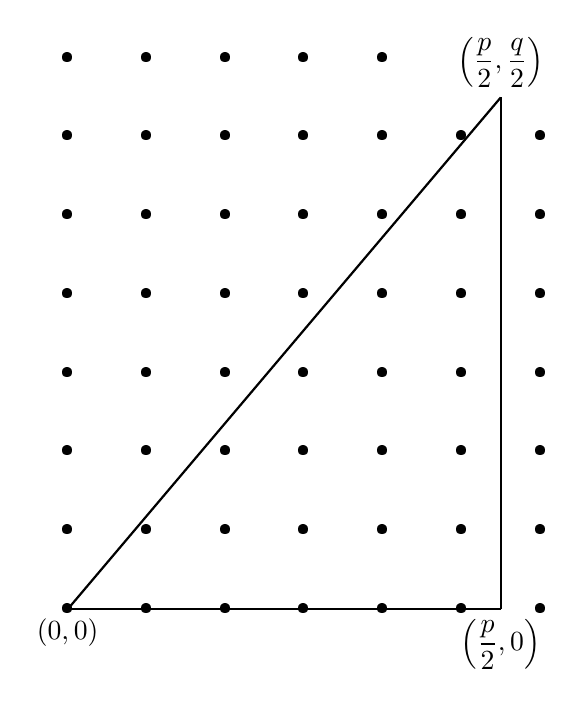
\begin{tikzpicture}
		\draw[thick] (0,0)--(5.5,6.5);
		\draw[thick] (5.5,6.5)--(5.5,0);
		\draw[thick] (0,0)--(5.5,0);

		\foreach \Point in {(0,0), (0,1), (0,2), (0,3), (0,4), (0,5), (0,6), (0,7),
			(1,0), (1,1), (1,2), (1,3), (1,4), (1,5), (1,6), (1,7),
			(2,0), (2,1), (2,2), (2,3), (2,4), (2,5), (2,6), (2,7),
			(3,0), (3,1), (3,2), (3,3), (3,4), (3,5), (3,6), (3,7),
			(4,0), (4,1), (4,2), (4,3), (4,4), (4,5), (4,6), (4,7),
			(5,0), (5,1), (5,2), (5,3), (5,4), (5,5), (5,6),
			(6,0), (6,1), (6,2), (6,3), (6,4), (6,5), (6,6)}{
			\node at \Point {\textbullet};
		}

		\node [below] at (0,0) {$(0,0)$};
		\node [below] at (5.5,0) {$\displaystyle\left(\frac{p}{2},0\right)$};
		\node [above] at (5.5,6.5) {$\displaystyle\left(\frac{p}{2},\frac{q}{2}\right)$};
		\end{tikzpicture}
	\end{center}

	The number of points with integer coordinates inside this triangle equals\[ \sum_{k=1}^{\frac{p-1}{2}} \Big\lfloor\frac{kq}{p} \Big\rfloor.\] You can easily verify this by using the fact that the hypotenuse of triangle lies on the line $y = \frac{q}{p}x$, and so the number of points with $x=k$ (where $1\leq k \leq \frac{p-1}{2}$) inside the triangle equals $\Big\lfloor\frac{kq}{p} \Big\rfloor$ (actually, we are counting the points vertically).

	Now consider the triangle with vertices on $(0,0), \left(0,q/2\right)$, and $\left(p/2,q/2\right)$.

	\begin{center}
		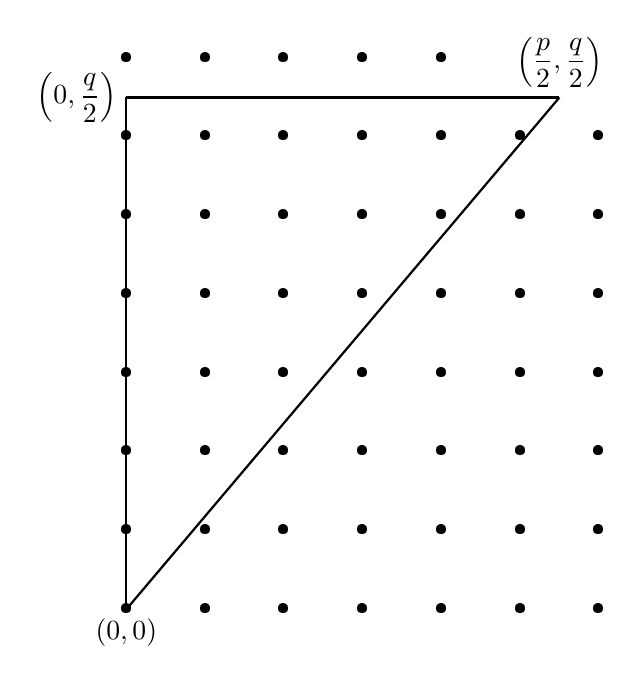
\begin{tikzpicture}

		\draw[thick] (0,0)--(5.5,6.5);
		\draw[thick] (5.5,6.5)--(0,6.5);
		\draw[thick] (0,0)--(0,6.5);

		\foreach \Point in {(0,0), (0,1), (0,2), (0,3), (0,4), (0,5), (0,6), (0,7),
			(1,0), (1,1), (1,2), (1,3), (1,4), (1,5), (1,6), (1,7),
			(2,0), (2,1), (2,2), (2,3), (2,4), (2,5), (2,6), (2,7),
			(3,0), (3,1), (3,2), (3,3), (3,4), (3,5), (3,6), (3,7),
			(4,0), (4,1), (4,2), (4,3), (4,4), (4,5), (4,6), (4,7),
			(5,0), (5,1), (5,2), (5,3), (5,4), (5,5), (5,6),
			(6,0), (6,1), (6,2), (6,3), (6,4), (6,5), (6,6)}{
			\node at \Point {\textbullet};
		}

		\node [below] at (0,0) {$(0,0)$};
		\node [left] at (0,6.5) {$\displaystyle\left(0,\frac{q}{2}\right)$};
		\node [above] at (5.5,6.5) {$\displaystyle\left(\frac{p}{2},\frac{q}{2}\right)$};
		\end{tikzpicture}
	\end{center}
	We can find the number of points with integer coordinates inside this triangle in a similar way to the previous one. This time, count the points horizontally and sum up the number of points with $y=1, y=2, \ldots$, and $y=\frac{p-1}{2}$. The result is \[ \sum_{k=1}^{\frac{q-1}{2}} \Big\lfloor\frac{kp}{q} \Big\rfloor.\]

	Now put these two triangles together to form a rectangle with vertices on $(0,0)$, $\left(0,q/2\right)$, $\left(p/2,0\right)$, and $\left(p/2,q/2\right)$.

	Let $x$ be number of the points with integer coordinates inside this rectangle. Obviously, $x$ is equal to the sum of such points in triangles (notice that since $p$ and $q$ are different, there is no point with integer coordinates on the hypotenuse of triangles). So
	\begin{align*}
	x = \sum_{k=1}^{\frac{p-1}{2}} \Big\lfloor\frac{kq}{p} \Big\rfloor+ \sum_{k=1}^{\frac{q-1}{2}} \Big\lfloor\frac{kp}{q} \Big\rfloor.
	\end{align*}
	According to lemma \eqref{lem:lawofqrlem2}, it follows that
	\begin{align}\label{eq:qrlawproof1}
	x \equiv \mu(q,p)+\mu(p,q) \pmod 2.
	\end{align}
	Let's count $x$ in another way.
	\begin{center}
		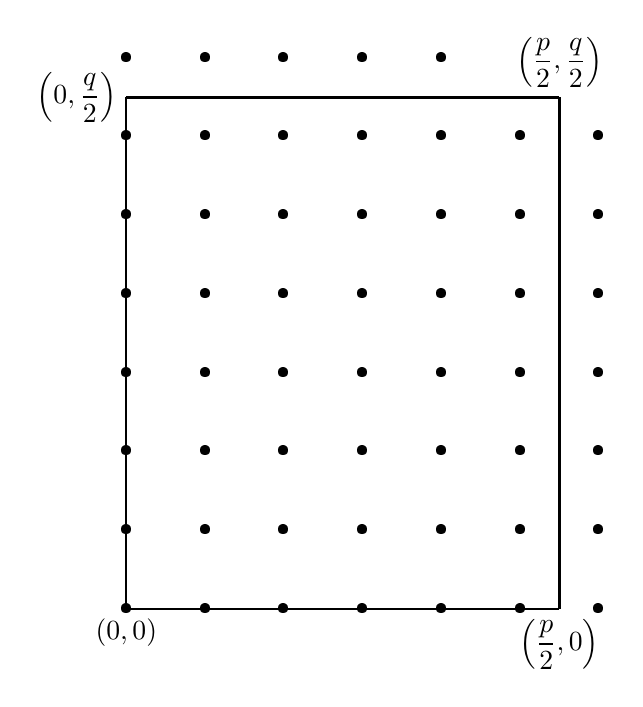
\begin{tikzpicture}
		\draw[thick] (5.5,6.5)--(5.5,0);
		\draw[thick] (0,0)--(5.5,0);
		\draw[thick] (5.5,6.5)--(0,6.5);
		\draw[thick] (0,0)--(0,6.5);

		\foreach \Point in {(0,0), (0,1), (0,2), (0,3), (0,4), (0,5), (0,6), (0,7),
			(1,0), (1,1), (1,2), (1,3), (1,4), (1,5), (1,6), (1,7),
			(2,0), (2,1), (2,2), (2,3), (2,4), (2,5), (2,6), (2,7),
			(3,0), (3,1), (3,2), (3,3), (3,4), (3,5), (3,6), (3,7),
			(4,0), (4,1), (4,2), (4,3), (4,4), (4,5), (4,6), (4,7),
			(5,0), (5,1), (5,2), (5,3), (5,4), (5,5), (5,6),
			(6,0), (6,1), (6,2), (6,3), (6,4), (6,5), (6,6)}{
			\node at \Point {\textbullet};
		}

		\node [below] at (0,0) {$(0,0)$};
		\node [left] at (0,6.5) {$\displaystyle\left(0,\frac{q}{2}\right)$};
		\node [below] at (5.5,0) {$\displaystyle\left(\frac{p}{2},0\right)$};
		\node [above] at (5.5,6.5) {$\displaystyle\left(\frac{p}{2},\frac{q}{2}\right)$};
		\end{tikzpicture}
	\end{center}
	Clearly, number of points with integer coordinates inside this rectangle is
	\begin{align}\label{eq:qrlawproof2}
	x=\Big\lfloor\frac{p}{2} \Big\rfloor \cdot \Big\lfloor\frac{q}{2} \Big\rfloor = \frac{p-1}{2}\cdot\frac{q-1}{2}.
	\end{align}
	Combining equations \eqref{eq:qrlawproof1} and \eqref{eq:qrlawproof2},
	\begin{align*}
	\mu(q,p)+\mu(p,q) \equiv \frac{p-1}{2}\cdot\frac{q-1}{2} \pmod 2.
	\end{align*}
	Now apply Gauss's criterion to finish the proof:
	\begin{align*}
	\left(\dfrac{p}{q}\right)\left(\dfrac{q}{p}\right) &=(-1)^{\mu(p,q)} \cdot (-1)^{\mu(q,p)} \\
	&= (-1)^{\mu(p,q)+\mu(q,p)}\\
	&=(-1)^{\frac{p-1}{2}\cdot\frac{q-1}{2}}.
	\end{align*}
\end{proof}

\end{document}